\subsection{PID-Regler}
\label{sec:PID-Regler}

Der PID-Regler ist eine essenzielle Komponente in der Automatisierungstechnik und wird zur Regelung verschiedener Prozessgrößen wie Geschwindigkeit, Temperatur und Spannung eingesetzt.

\paragraph{Proportionalanteil (P)} \mbox{}\\
Der Proportionalanteil reagiert direkt auf den aktuellen Fehlerwert \( e(t) \), indem er diesen mit der Proportionalverstärkung \( K_p \) multipliziert:
\begin{equation}
P_{\text{out}} = K_p \cdot e(t)
\end{equation}

\paragraph{Integralanteil (I)} \mbox{}\\
Der Integralanteil akkumuliert kontinuierlich die Fehlerwerte und multipliziert das Ergebnis mit der Integralverstärkung \( K_i \), um den kumulierten Fehler zu korrigieren:
\begin{equation}
I_{\text{out}} = K_i \cdot \int e(t) \, dt
\end{equation}

\paragraph{Differentialanteil (D)} \mbox{}\\
Der Differentialanteil betrachtet die Änderungsrate des Fehlers und multipliziert sie mit der Differentialverstärkung \( K_d \):
\begin{equation}
D_{\text{out}} = K_d \cdot \frac{d}{dt} e(t)
\end{equation}

\paragraph{PID-Regelungsgleichung} \mbox{}\\
Diese drei Anteile kombiniert ergeben den gesamten Steuerausgang des PID-Reglers:
\begin{equation}
\text{Steuerausgang} = P_{\text{out}} + I_{\text{out}} + D_{\text{out}}
\end{equation}

\paragraph{Einstellung der Verstärkungsfaktoren} \mbox{}\\
Die sorgfältige Einstellung der Verstärkungsfaktoren \( K_p, K_i, \) und \( K_d \) ist entscheidend, um eine optimale Systemleistung zu erzielen.

\paragraph{Anwendung bei Gleichstrom-Gleichstrom-Wandlern} \mbox{}\\
PID-Regler werden verwendet, um die Ausgangsspannung von DC-DC-Wandlern zu stabilisieren, indem sie ständig die Ist-Spannung mit der Soll-Spannung vergleichen und entsprechend regulieren.
\cite{SwainBaid2014}

\paragraph{Fazit} \mbox{}\\
Der PID-Regler ist aufgrund seiner Effizienz und Anpassungsfähigkeit für eine Vielzahl von Anwendungen geeignet.

\begin{figure}[htbp]
    \centering
    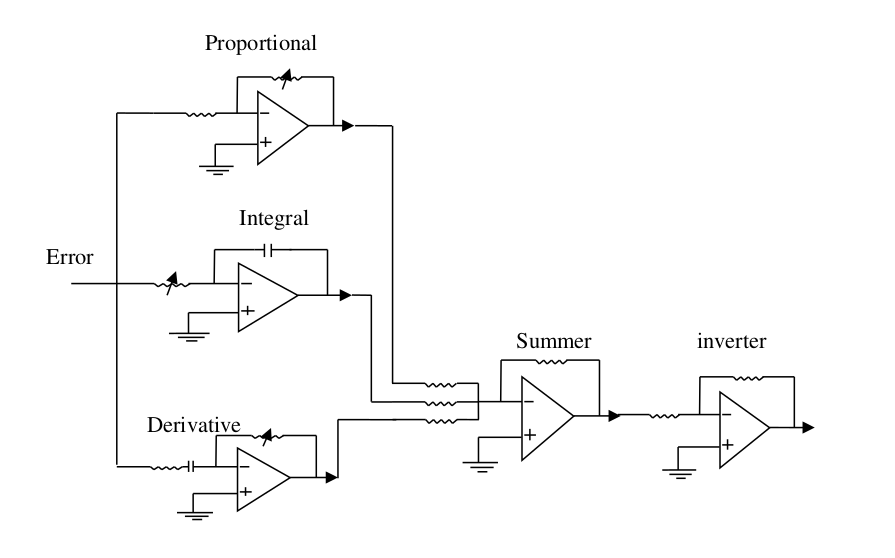
\includegraphics[width=0.6\linewidth]{2Grundlagen/13PID.png}
    \caption{Schematische Darstellung eines PID-Regler. Quelle: \cite{SwainBaid2014}}
    \label{fig:PID_converter}
\end{figure}

\paragraph{Zusammenfassung der PID-Reglerkomponenten} \mbox{}\\
Der PID-Regler passt das Systemverhalten durch die proportionale, integrale und differenzielle Reaktion auf Fehlerwerte an. Die Zusammenarbeit dieser drei Komponenten sorgt für ein ausgewogenes und effektives Regelungssignal.


